\chapter{Intellectual Property}

\section{Setting}

OpenCombat takes place in a fantasy world with modern amenities.

\section{Tone}

\begin{description}
    \item[Light-Hearted] The intellectual property should be relatable and not too emotionally taxing.
    \item[Comical] The property should emphasis humor and enjoyment.
    \item[Raunchy] Characters can have little-to-no language filter.
\end{description}

\section{Overview}

Prosperity is a bustling cityscape populated by fantasy creatures of all shapes and sizes. The city's newest attraction is a large arena with plentiful seating and amenities funded by one of the city's monopolists. To celebrate the grand opening, the arena is hosting the city's first ever combat tournament. People from all walks of life have flocked to the city to either prove they have what it takes to win or to watch the spectacle. As the player progresses through the tournament, they discover that the monopolist and his cohorts are stealing the powers away from the most powerful defeated combatants and trying to mass-produce them as consumable potions. The player will ultimately stop the company and become the first champion of the tournament.

\section{Conflict}

\paragraph{} There are two central conflicts in the narrative:

\begin{enumerate}
    \item Competing against others to become the first tournament champion.
    \item Stopping the monopolist from selling the powers of defeated combatants.
\end{enumerate}

\section{The World}

\subsection{Outside Prosperity}

\paragraph{} The world outside the walls of Prosperity is in a state of massive change. For as long as history has been recorded, kings and emperors ruled over their race and any races from kingdoms they had conquered. This system fell apart, however, 15 years ago when the human kingdom invaded the orc kingdom and started the the War of Warm Thrones named because poor people were being sent off to fight and die while kings and nobles were able to stay home. After every other world power, except the Republic of Prosperity, joined in the conflict and after 5 years of stalemates and pointless violence, the citizens of the world became tired of killing their neighbors. The conscripts rose up, ending the war between the kingdoms but starting new ones inside each kingdom.

\paragraph{} The rebellion that resulted from the War of Warm Thrones resulted in a shift in the geopolitics of the world. The gnome and dwarf kingdoms were the first to fall, being replaced with an autocratic communist state called The Tinkerer's Commune. After the orc kingdom fell to a nationalist military dictatorship and became The Dawning Empire, the troll and goblin kingdoms were quickly absorbed. The human kingdom, meanwhile, was able to survive but only if the king was willing to adopt a constitution which, alongside the Elf and Goliath kingdoms, formed The Commonwealth. The kingdoms of the corgos, purrs, kongs and drakes united during the war and became the Imperium Animalia.

\subsection{Prosperity Itself}

\paragraph{} The Republic of Prosperity is a bustling city-state that allures people from around the world with its promise of a fresh start and opportunity for all. Legend has it that the city was founded around 200 years in the past by humble merchants from various kingdoms who were so sick of having to deal with unreasonable and unfair taxation; this led the dwarven merchant Lorenzo Wealthcovet to buy the land where the city-state sits today. Historians, however, question the authenticity of the legend and argue that Wealthcovet and the other merchants avoided taxation not because they thought the taxes were unfair but rather that they wanted more power within the kingdoms and the monarchs denied them.

\paragraph{} The city itself is a bustling cityscape with a vibrant nightlife, diverse populace and modern amenities. After the War of Warm Thrones, the city became a place for refugees, deserters and merchants to come and continue on with a quiet and peaceful life. The streets of the central district are lined with jazz bars, small stores and lavish hotels. After the sun sets, the bars are filled with patrons from around the world and all different walks of life. The city's business tycoons, a group of self-made people and inherited wealth, own the vast majority of the businesses in the district as well as the businesses that serve the needs of those businesses such as distilleries, cleaning services and protection services.

\paragraph{} What the historians and common folk of Prosperity can agree on is that the city-state does not live up to its name. Business tycoons own massive monopolies that use their capital to bribe government officials, get lucrative contracts and enrich themselves at the expense of society. Most of the working class people in Prosperity work for the city's monopolists and although they put on a smile when they work the central district, they leave tired and underpaid. The corruption and neglect in Prosperity's poorest neighborhoods is so rampant that organized crime has been able to take over the streets. This is the backdrop behind which the new arena is being built.

\section{Races}

\subsection{Gnomes}

\paragraph{} The gnomes are a short people who populate hills, forests and caves alongside the drawves. A humble people, they are best known as being the punchline in jokes made about height. What they do not have in size, however, they make up for with their wit. Most gnomes pursue higher education such as engineering or magic school while the most brave learn the art of combat despite their size disadvantage.

\subsection{Dwarves}

\paragraph{} A proud and noble race, these long-bearded, stout people developed the Berserker fighting style and have since exported it to the world. Like their gnomish cousins, dwarves primarily live in mountainous areas. On average, most dwarves like to pursue blacksmithing or military service however some choose to pursue the life of the Monk.

\subsection{Goblins}

\paragraph{} These plains people are best known for their short stature and long ears. Traditionally merchants, Goblins are also well known for their exceptional sense of fashion and engineering skills. Unlike other races of their size, they prefer to live in flatlands where they can build trading posts and small towns.

\subsection{Corgos}

\paragraph{} The small Corgi people are known as being the most adorable people on the planet but also the most peaceful. Before it was absorbed into Imperium Animalia, the kingdom of the Corgos had only use their Monk fighting style to defend their homes. The most notable contribution to the world was Zen Grass, a plant that is smoked and consumed for medical or recreational purposes. Most Corgos pursue the ways of the Monk but also have a strong tradition of cooking and performance art.

\subsection{Humans}

\paragraph{} The most populace of all the races, humans lived all across the world but were largely centered around rivers and lakes. Arrogant yet driven, humans pride themselves on overcoming any obstacles that lie before them. Humans have a broad range of occupations they typically pursue but they are most often sailors, mages, musicians and politicians.

\subsection{Orcs}

\paragraph{} The orcs originated from complex cave societies and developed a culture that valued strength as well as honor. Primarily miners, blacksmiths and military officers, orcs are exceptional at physical tasks and also make for expert builders. Their architecture, monuments and other constructs have served as inspiration for other societies around the world.

\subsection{Elves}

\paragraph{} The race that introduced magic to the world, elves are an elegant people that originated from mountainous regions. Known for their goldsmithing, jewelry and art, the elves also mastered the arcane arts and were pacifistic. Today, most elves are academics, adventurers and can often be tending the wounded as nurses or doctors.

\subsection{Purrs}

\paragraph{} The feline people of the Purrs thrived in jungles alongside the kongs for most of recorded history. Quick, nimble and intelligent, purrs built their societies in the canopies of the trees and are considered to have a strong engineering tradition. In modern times, purrs expert building skills make them great sailors.

\subsection{Kong}

\paragraph{} The large, gorilla people of the jungle lived alongside the purrs in peace for most of recorded history. Like the purrs, they also lived in treetop societies however their constructions were much larger and utilitarian than the purrs' elegant designs. They were the race that spread the Druid arts to the world and today largely serve as Druids, builders, bodyguards and academics.

\subsection{Trolls}

\paragraph{} Trolls are most well-known for two things: their tusks and their size. These towering being are close cousins of the orcs and also lived in cave societies. Their raw strength makes them most suitable for mining, building, blacksmithing and military service but they are also proud writers and artisans. Their blacksmithing abilities have allowed them to create resilient but heavy armor that is used by the strong races of the world.

\subsection{Goliaths}

\paragraph{} These towering cousins to humans have lived along them on river settlements that were peaceful and prosperous. Despite their size, goliaths prefer to stay out of combat and focus on the arts, woodworking, construction and cooking. There is a strong tradition of Druids in early goliath societies as well but those who served in combat often did so as heavily-plated fighters.

\subsection{Drakes}

\paragraph{} Bearing a striking resemblance to dragons, Drakes are more humanoid than their look-alike and also do not have wings. They also lived atop the mountains like the Corgo did however they were never able to successful capture any Corgo lands. Although the Drake tradition emphasizes war, not all take the path of their claymore-wielding ancestors; some have chosen to live peaceful lives as Druids, merchants and stonemasons.

\section{Non-playable Characters}

\subsection{Molten Mic}

\begin{description}
    \item[Race] Mech
    \item[Gender] N/A
    \item[Age] 12  
\end{description}

\subsubsection{Physical Appearance}

\begin{description}
    \item[Height] 6ft, 7in.
    \item[Weight] 637lbs
\end{description}

\subsubsection{Characteristics}

\begin{itemize}
    \item He has veins filled with lava.
    \item His eyes glow orange from the lava-flow.
    \item His metal plating is black and thick with cracks that show the light from the flowing lava.
    \item His big belly is engineered to also serve as a speaker.
\end{itemize}

\subsubsection{Personality}

\begin{itemize}
    \item Outspoken
    \item Blunt
    \item Prideful
    \item Sarcastic
    \item Humorous
\end{itemize}

\subsubsection{Background}

\paragraph{} Molten Mic is an award winning rapper and activist best known for his hit singles \textit{Zen Grass and Goliath Ass}, \textit{No Shame} and \textit{masters = null;}. Constructed as a speaker mech for a dwarven rap duo, Molten Mic escaped servitude and took to the underground rap scene in Prosperity. His flows spoke to the working class people of Prosperity and he would eventually become the most popular rapper in the city. When he is not rapping, Molten Mic is a advocate for mech rights and the rights of the working class people in Prosperity.

\subsubsection{Role}

\paragraph{} Molten Mic was hired by Mr. Peels to be the first commentator in the tournament's history. His rough-around-the-edges style makes him a fan favorite and his commentary is legendary. Molten Mic has no problem using his podium to say exactly what he thinks about the match. Some of the comments he will make in-match include:

\begin{itemize}
    \item "Holy shit, leave the little one alone!"
    \item "G.O.N.E. GONE!"
    \item "That combo was some fresh shit!"
    \item "Damn, my ass could feel that from up here and I don't have nerves."
    \item "Now THAT is an ass-whooping."
    \item "They don't pay me to talk about y'all wasting time; attack each other, dammit!"
    \item "Good thing I didn't bet my mortgage on \textit{that} one."
    \item "Do it to 'em!"
    \item "Whoever tossed that Zen Grass into the arena: bring some up to the podium, please and thank you."
\end{itemize}

\subsection{Eugene Esquire Peels IV}

\begin{description}
    \item[Race] Kong
    \item[Gender] Male
    \item[Age] 36  
\end{description}

\subsubsection{Physical Appearance}

\begin{description}
    \item[Height] 6ft, 2in.
    \item[Weight] 512lbs
\end{description}

\subsubsection{Characteristics}

\begin{itemize}
    \item He always dresses up in a button-up shirt with a tie.
    \item He is almost always smiling.
    \item His fur is dark grey and very finely groomed.
\end{itemize}

\subsubsection{Personality}

\begin{itemize}
    \item Polite
    \item Elitist
    \item Snobby
    \item Intelligent
    \item Studious
\end{itemize}

\subsubsection{Background}

\paragraph{} Born into the the wealthy Peels family, Eugene inherited the Peels Corporation empire after his parents mysteriously died in an accident. Quiet and studious, his education that the best schools in Prosperity prepared him well for the task of owning the entertainment monopoly his parents left behind. He is also known for his extension philanthropy which prominent journalists in the city have accused of being a front for bribery and money laundering schemes. Like his parents and all the other monopolists in Prosperity, Eugene's only goal is to become the richest man in the world and he will stop at nothing to achieve that.

\subsubsection{Role}

\paragraph{} As the owner of the new arena, Mr. Peels will guide the player through the main menu the first time they log in. He also will tell the player about any announcements about the game or upcoming events. He is also the default playable large character if the player has no custom characters of that size.

\subsection{De'Dra Orgur}

\begin{description}
    \item[Race] Troll
    \item[Gender] Female
    \item[Age] 65  
\end{description}

\subsubsection{Physical Appearance}

\begin{description}
    \item[Height] 6ft, 5in.
    \item[Weight] 505lbs
\end{description}

\subsubsection{Characteristics}

\begin{itemize}
    \item Her skin is dark-purple will several moles and age-spots.
    \item She got her tusks pierced when she was younger but now keeps it classy within minimal tusk-rings or other jewelry.
    \item She always seems to be glaring at others.
    \item She also always seems to be expressionless; it is unclear whether she is apathetic or bottling in rage.
\end{itemize}

\subsubsection{Personality}

\begin{itemize}
    \item Grouchy
    \item Focused
    \item Motherly
    \item Merciless
\end{itemize}

\subsubsection{Background}

\paragraph{} De'Dra is a troll born and raised in Prosperity. She started off as a waitress at one of the city's upscale jazz bars. She caught the attention of Mr. Peels who hired her as his personal secretary after scaring some drunkards into paying a bill they were refusing to pay. She does not tolerate incompetence or mistakes which is why Mr. Peels put her in charge of the tournament's logistics.

\subsubsection{Role}

\paragraph{} De'Dra will be the player's guide through the settings and their account information. She will inform the player of how the account system works as well as give recommendations for the settings players should use.

\subsection{Lola Moonborn}

\begin{description}
    \item[Race] Elf
    \item[Gender] Female
    \item[Age] 31  
\end{description}

\subsubsection{Physical Appearance}

\begin{description}
    \item[Height] 5ft, 5in.
    \item[Weight] 120lbs
\end{description}

\subsubsection{Characteristics}

\begin{itemize}
    \item Unlike most other elves, she has a slight tan from working outside all day.
    \item She is very physically fit; her six-pack and muscles make her intimidating to criminals on the street.
    \item Her police uniform is ripped and tattered but she refuses to get a new one.
    \item The rumor among criminals is that her bright green eyes glow in the dark but that is just a myth.
\end{itemize}

\subsubsection{Personality}

\begin{itemize}
    \item Kind
    \item Hard-working
    \item Stubborn
    \item Tenacious
\end{itemize}

\subsubsection{Background}

\paragraph{} Lola Moonborn embodied the Prosperity Dream; born into deep poverty, she taught herself magic and became a police officer. While on the job, she was notorious among crooks and thieves as one of the only cops in the city that both would not take bribes and destroy them if they tried to offer. She is considered to be a hero among the working class of the city but her investigative tendencies have made her the enemy of powerful people. Suspecting Mr. Peels is up to something, she decided to enter the tournament and investigate.

\subsubsection{Role}

\paragraph{} Lola will help the player through the tutorial of the game as well as in training mode. She is also the default playable medium character if the player has no custom characters of that size.

\subsection{Rufus Wigglebottom}

\begin{description}
    \item[Race] Corgo
    \item[Gender] Male
    \item[Age] 31  
\end{description}

\subsubsection{Physical Appearance}

\begin{description}
    \item[Height] 3ft, 3in.
    \item[Weight] 70lbs
\end{description}

\subsubsection{Characteristics}

\begin{itemize}
    \item He has bright orange fur with white dimples and big cheeks.
    \item His eyes are a soulless brown that is contrasted by his bright smile.
    \item He equipped his police uniform with Monk gliders so he can fight crime from the skies.
\end{itemize}

\subsubsection{Personality}

\begin{itemize}
    \item Kind
    \item Sassy
    \item Determined
    \item Vicious
    \item Relentless
\end{itemize}

\subsubsection{Background}

\paragraph{} One of the most adorable member of the police force, Rufus has been a deputy since after learning the ways of the Monk. He grew up homeless and alone most of his life until Lola saved him from a group of muggers trying to shake him down for all he had. Her courage inspired him to learn how to fight and after learning how he came back to the streets where he was mugged and began a vicious campaign of vigilante justice against the criminals. Impressed with his willingness to shameless beat criminals, Lola brought him on as a partner and the two have been best friends ever since.

\subsubsection{Role}

\paragraph{} Rufus will guide the player through creating their own combatants. He motivates them to make their character however they want and to do great in the arena. He is also the default playable small character if the player has no custom characters of that size.

\section{Visual References}

\subsection{Characters}

\begin{figure}[h!]
    \centering
    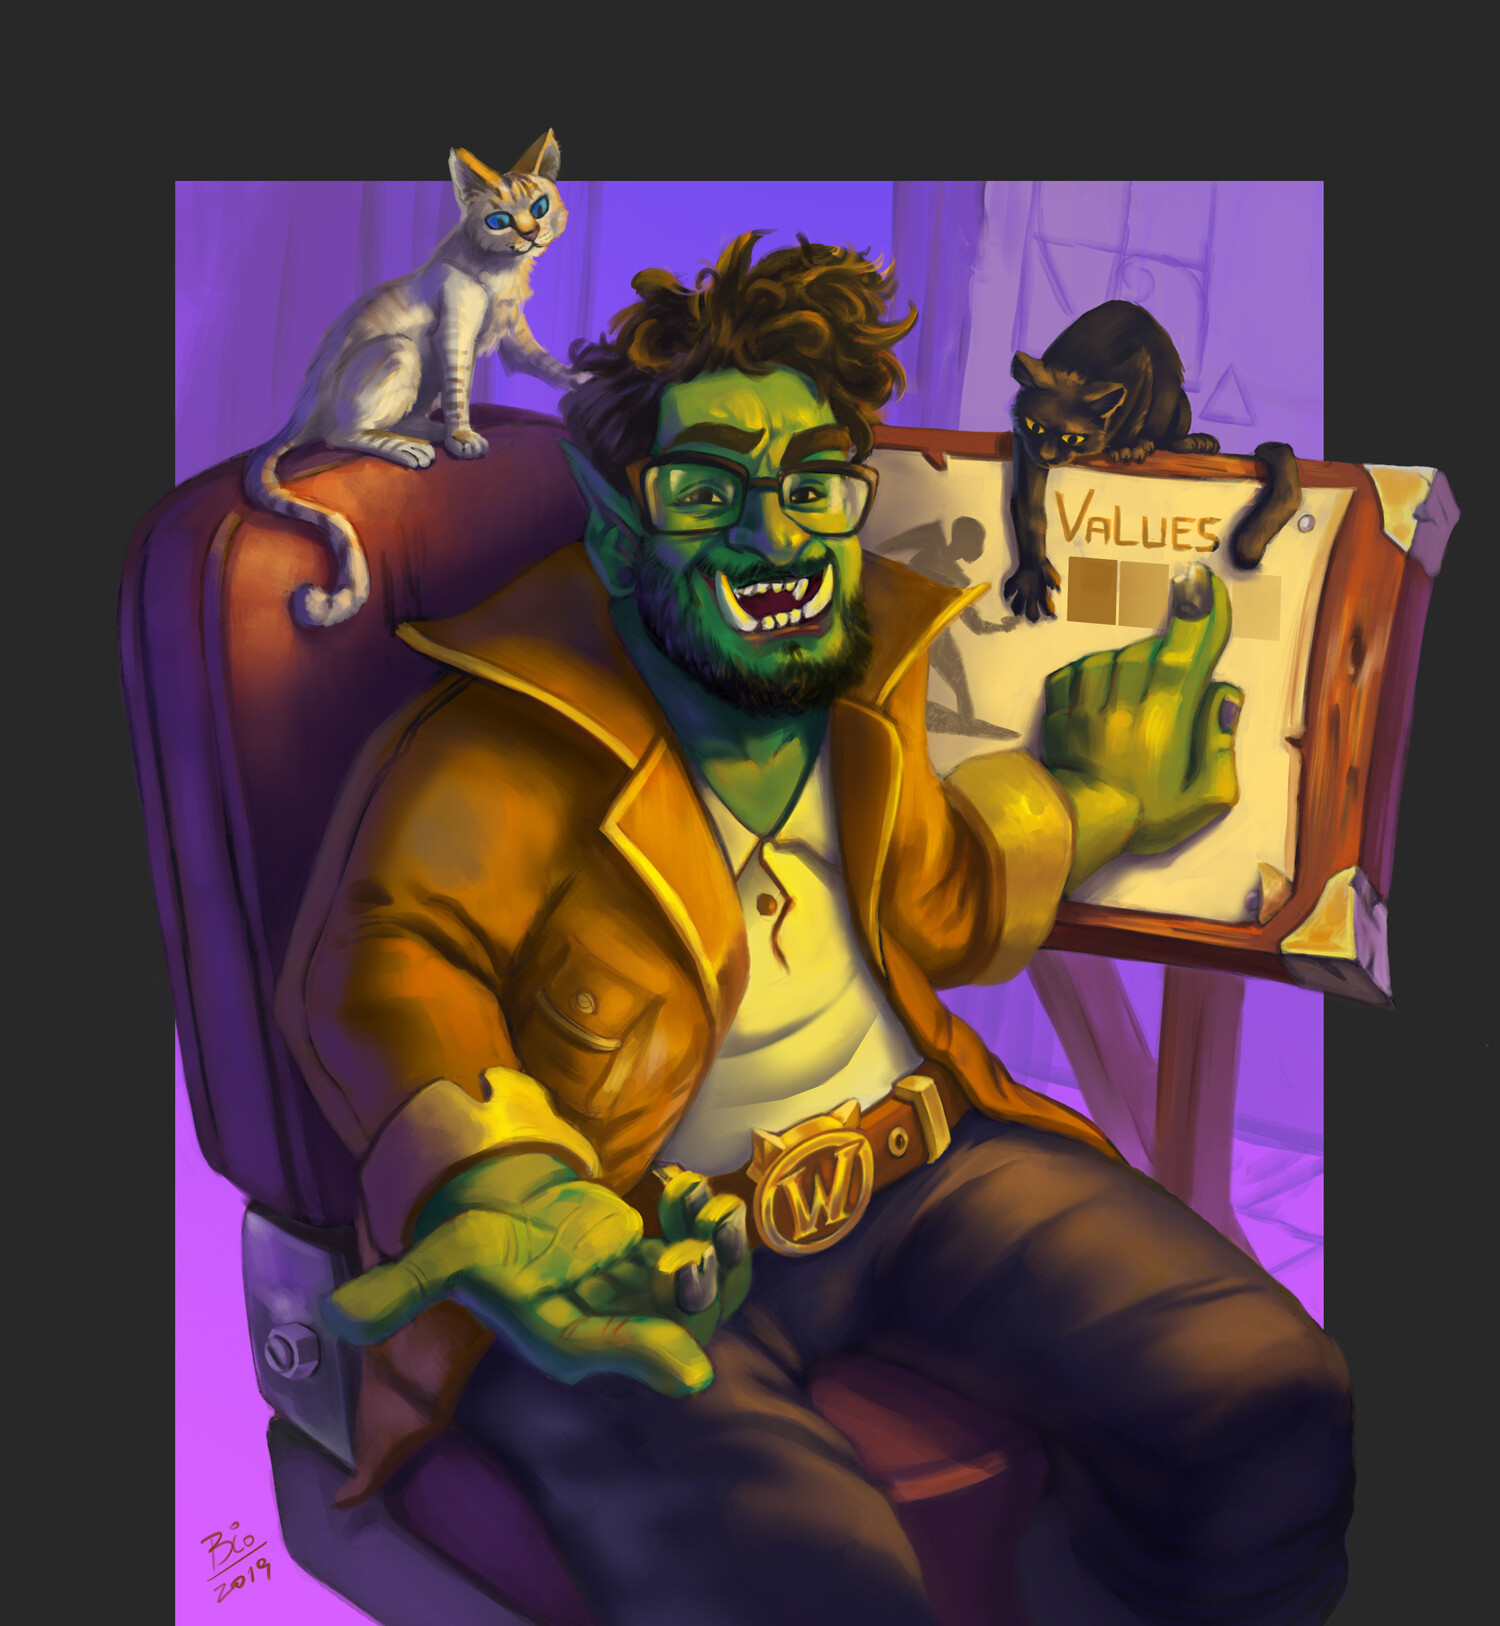
\includegraphics[width=0.4\linewidth]{images/characters-civilian.jpg}
    \caption{Cesar, The Mentor by Murillo Ribeiro. \nocite{ribeiro_cesar_2019}}
\end{figure}

\begin{figure}[h!]
    \centering
    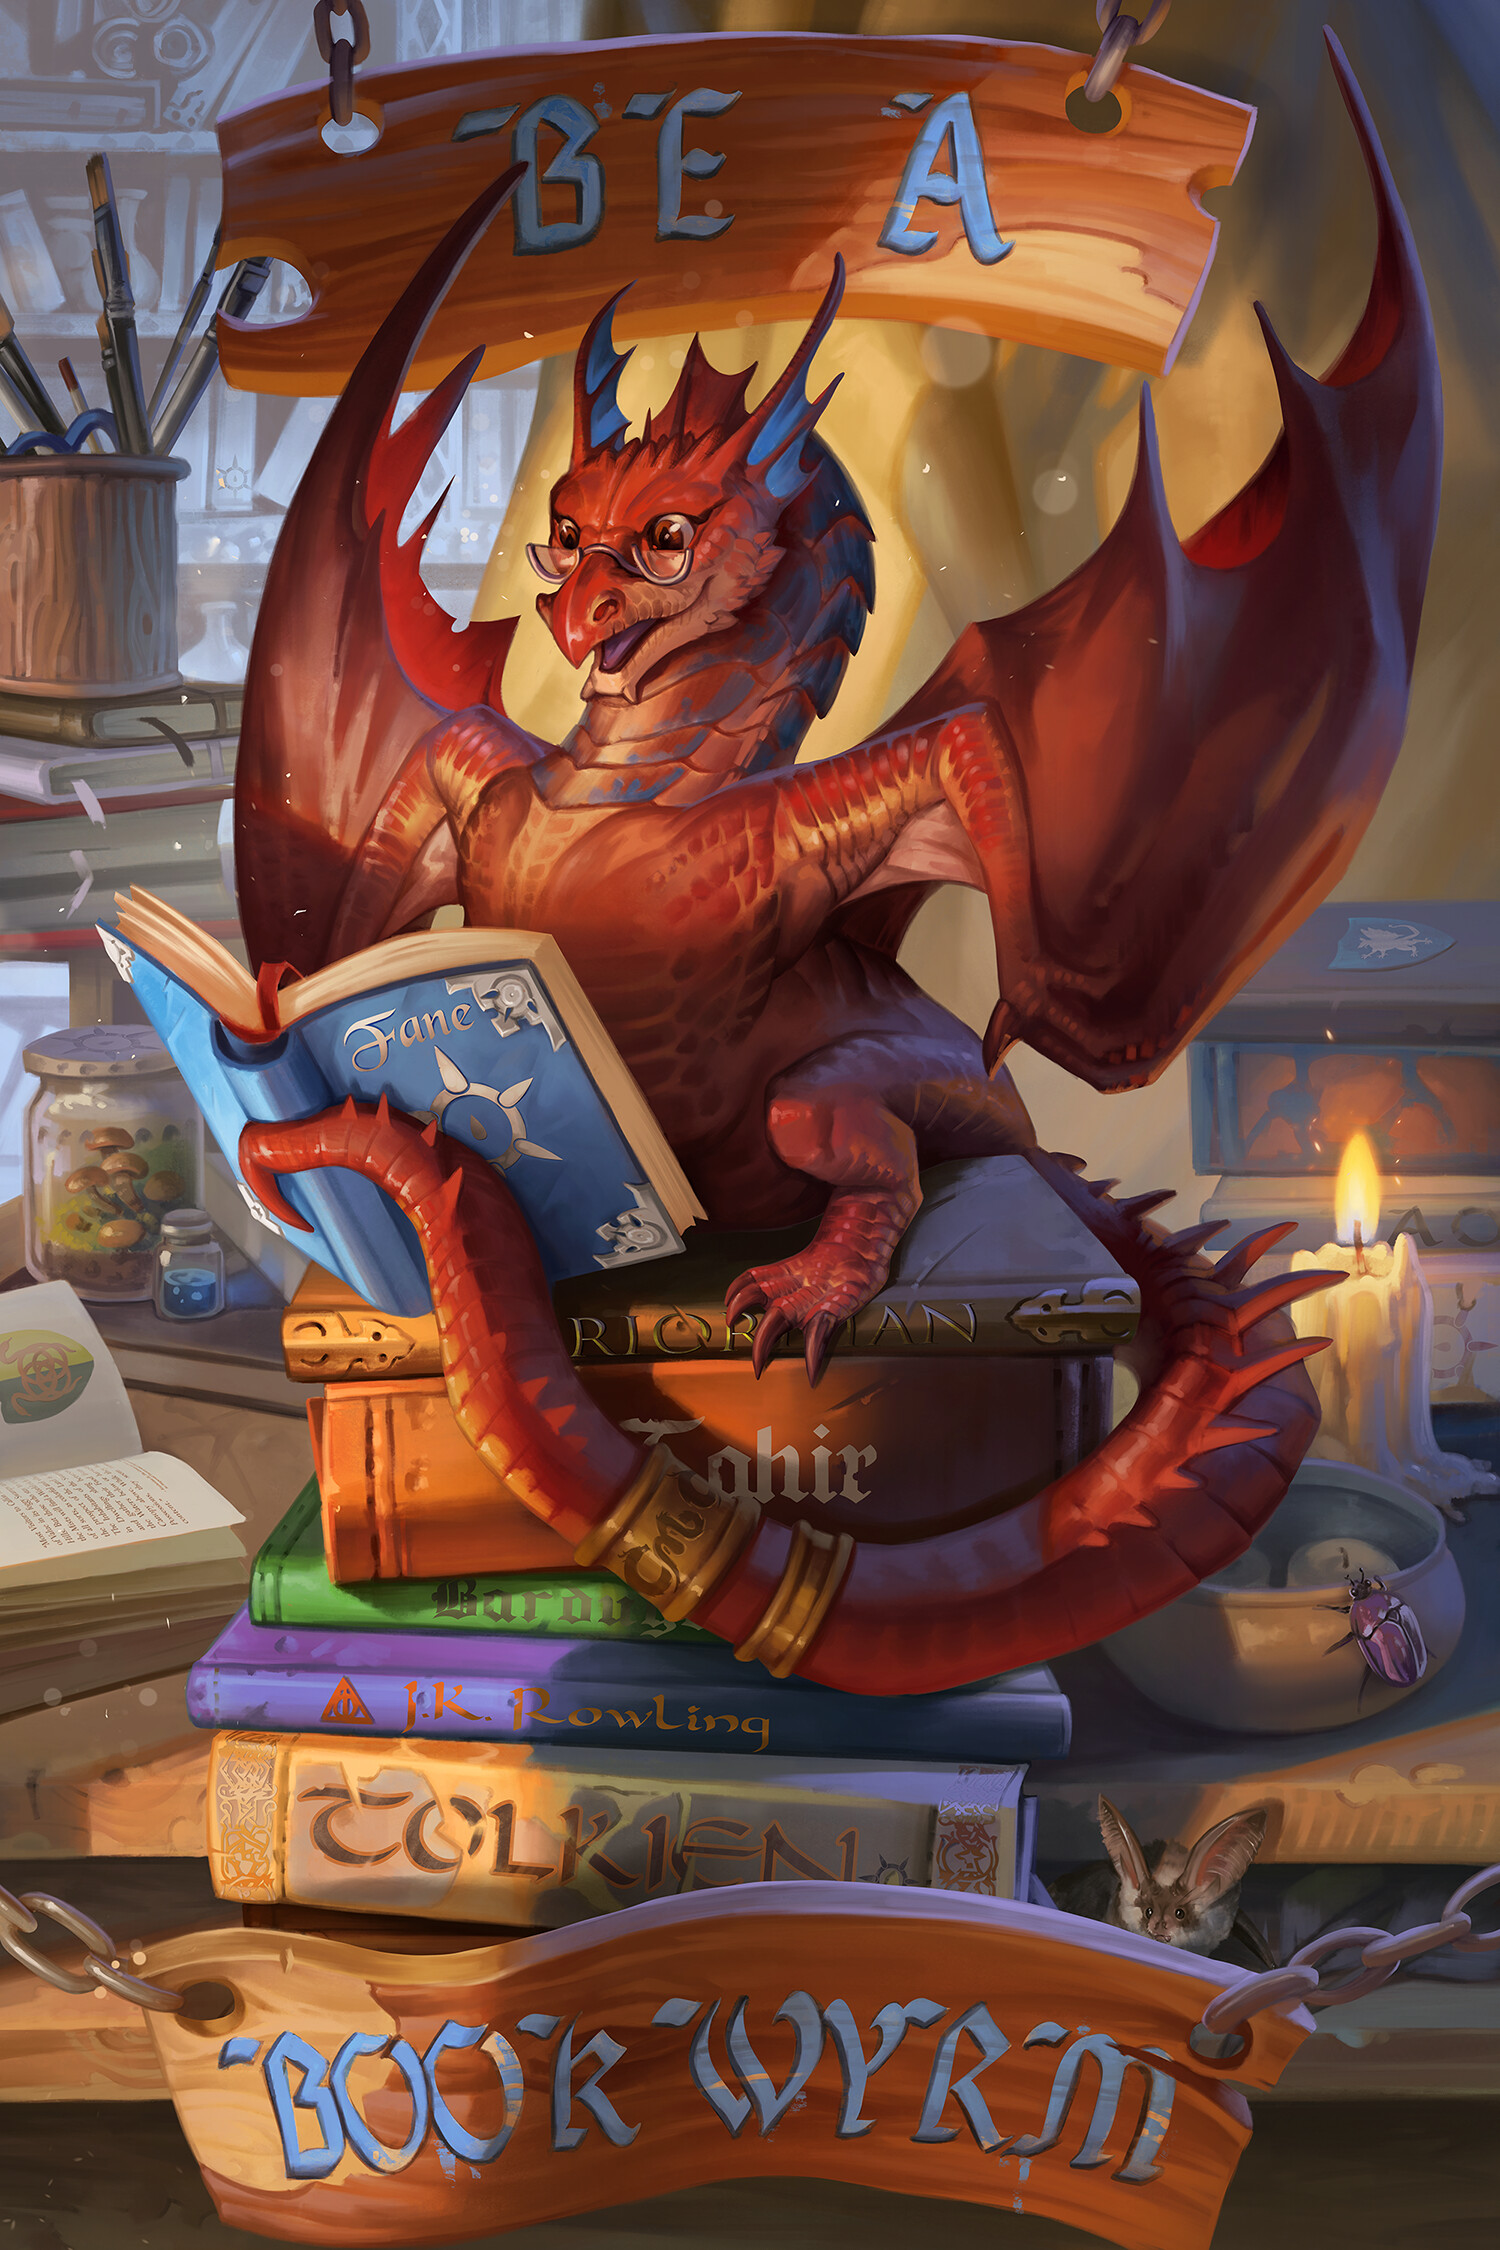
\includegraphics[width=0.3\linewidth]{images/characters-dragon.jpg}
    \caption{Book Wyrm by Milica \v{C}elikovi\'{c}.\nocite{celikovic_book_2019}}
\end{figure}

\begin{figure}[h!]
    \centering
    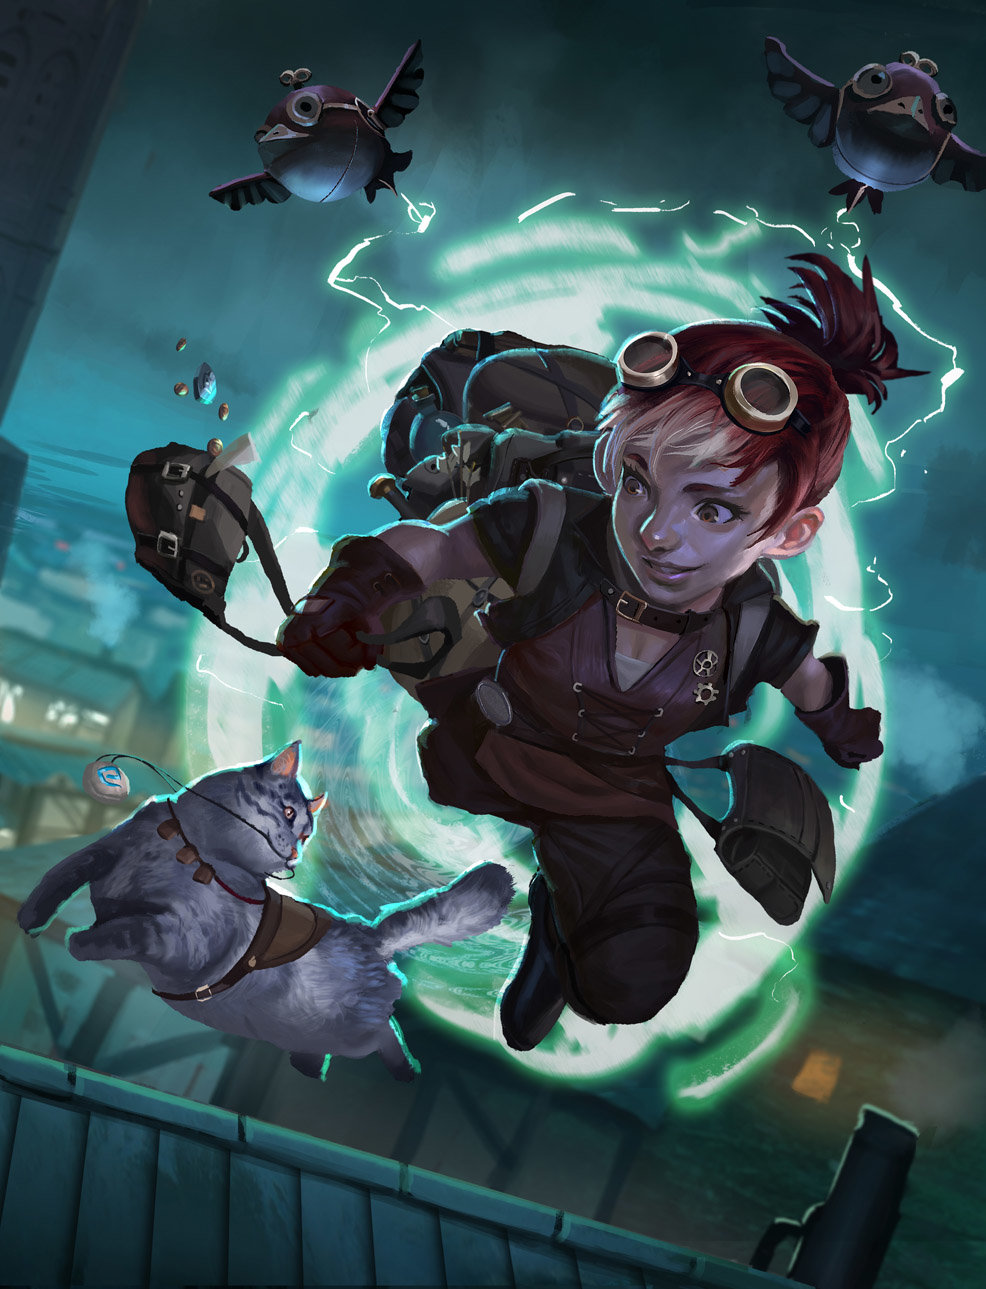
\includegraphics[width=0.3\linewidth]{images/characters-gnome.jpg}
    \caption{Hearthstone Challenge "Zapping Bird" by Hendry Iwanaga.\nocite{iwanaga_hearthstone_2015}}
\end{figure}

\begin{figure}[h!]
    \centering
    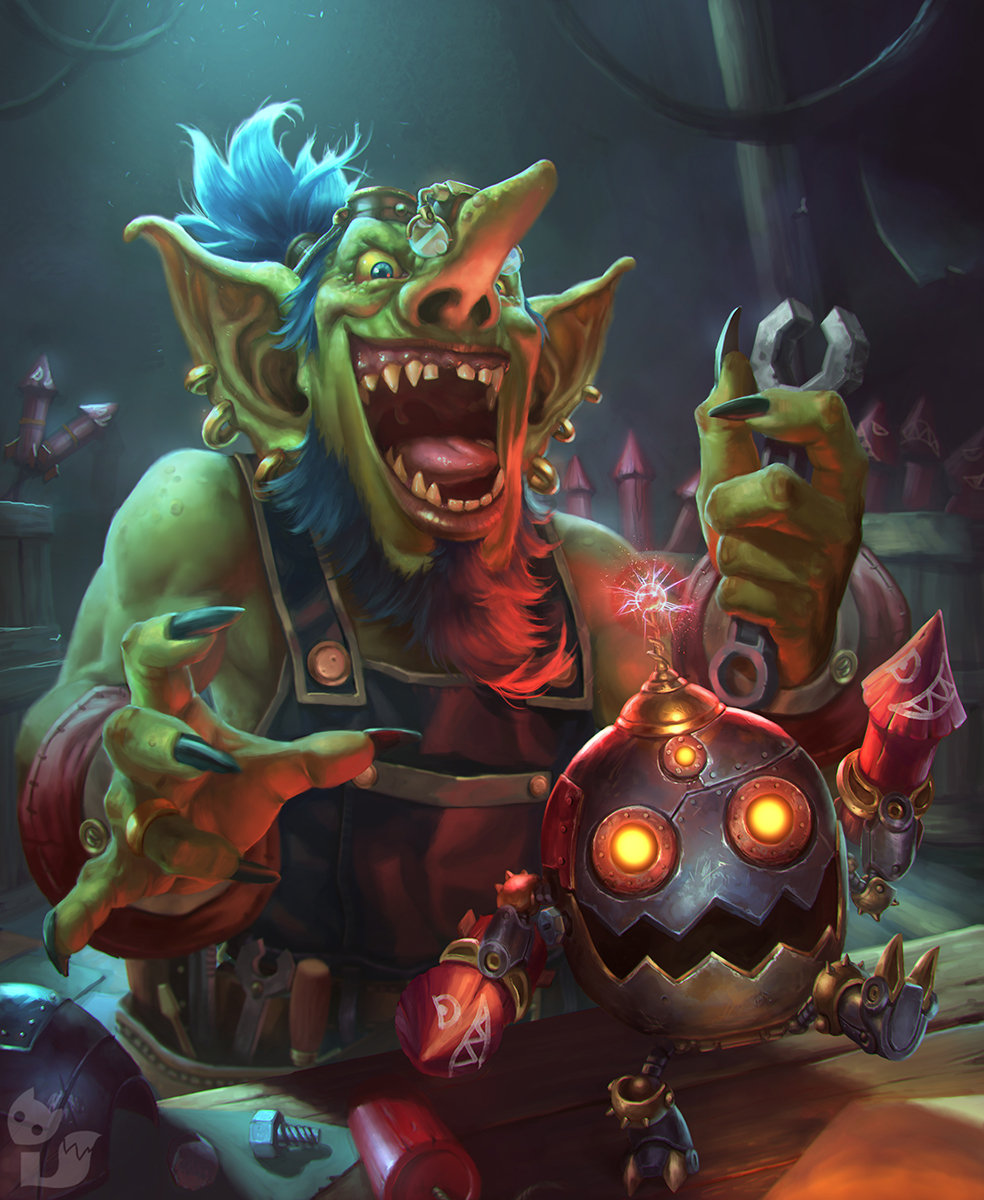
\includegraphics[width=0.3\linewidth]{images/characters-goblin.jpg}
    \caption{Mad Goblin Technician by Lie Setiawan.\nocite{setiawan_mad_2015}}
\end{figure}

\begin{figure}[h!]
    \centering
    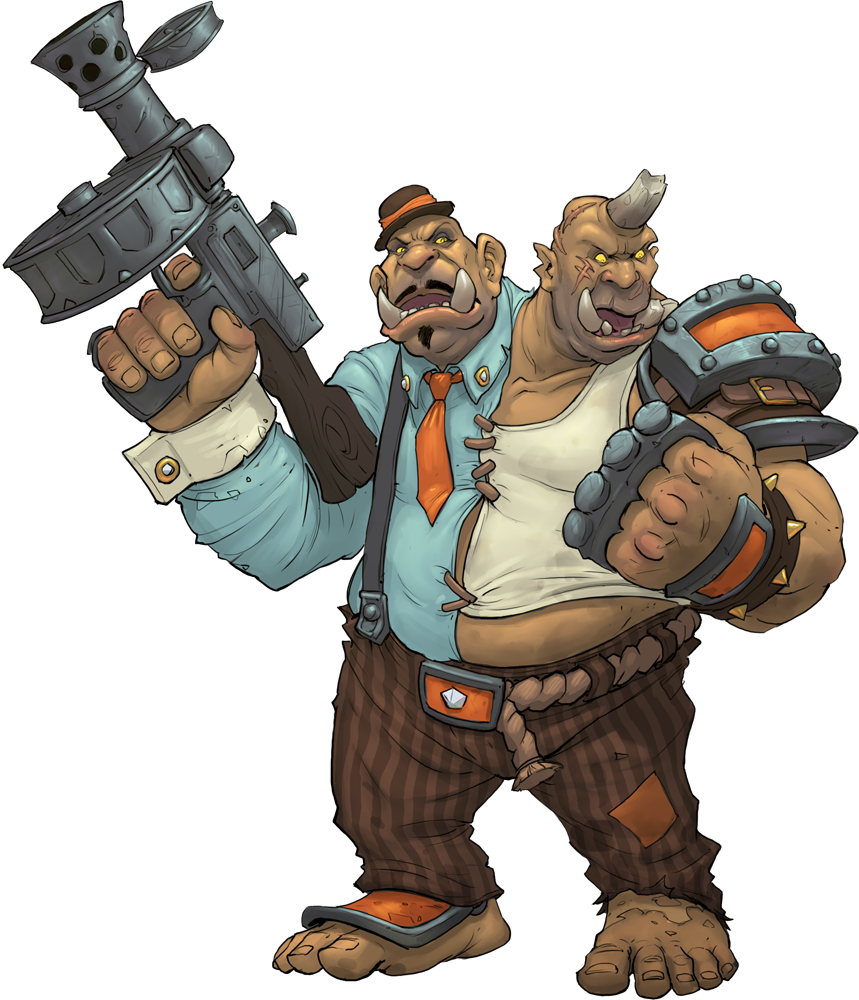
\includegraphics[width=0.3\linewidth]{images/characters-balance.png}
    \caption{Don Han'Cho by Blizzard Entertainment, Inc.\nocite{blizzard_entertainment_inc_don_2016}}
\end{figure}

\subsection{Location}

\begin{figure}[h!]
    \centering
    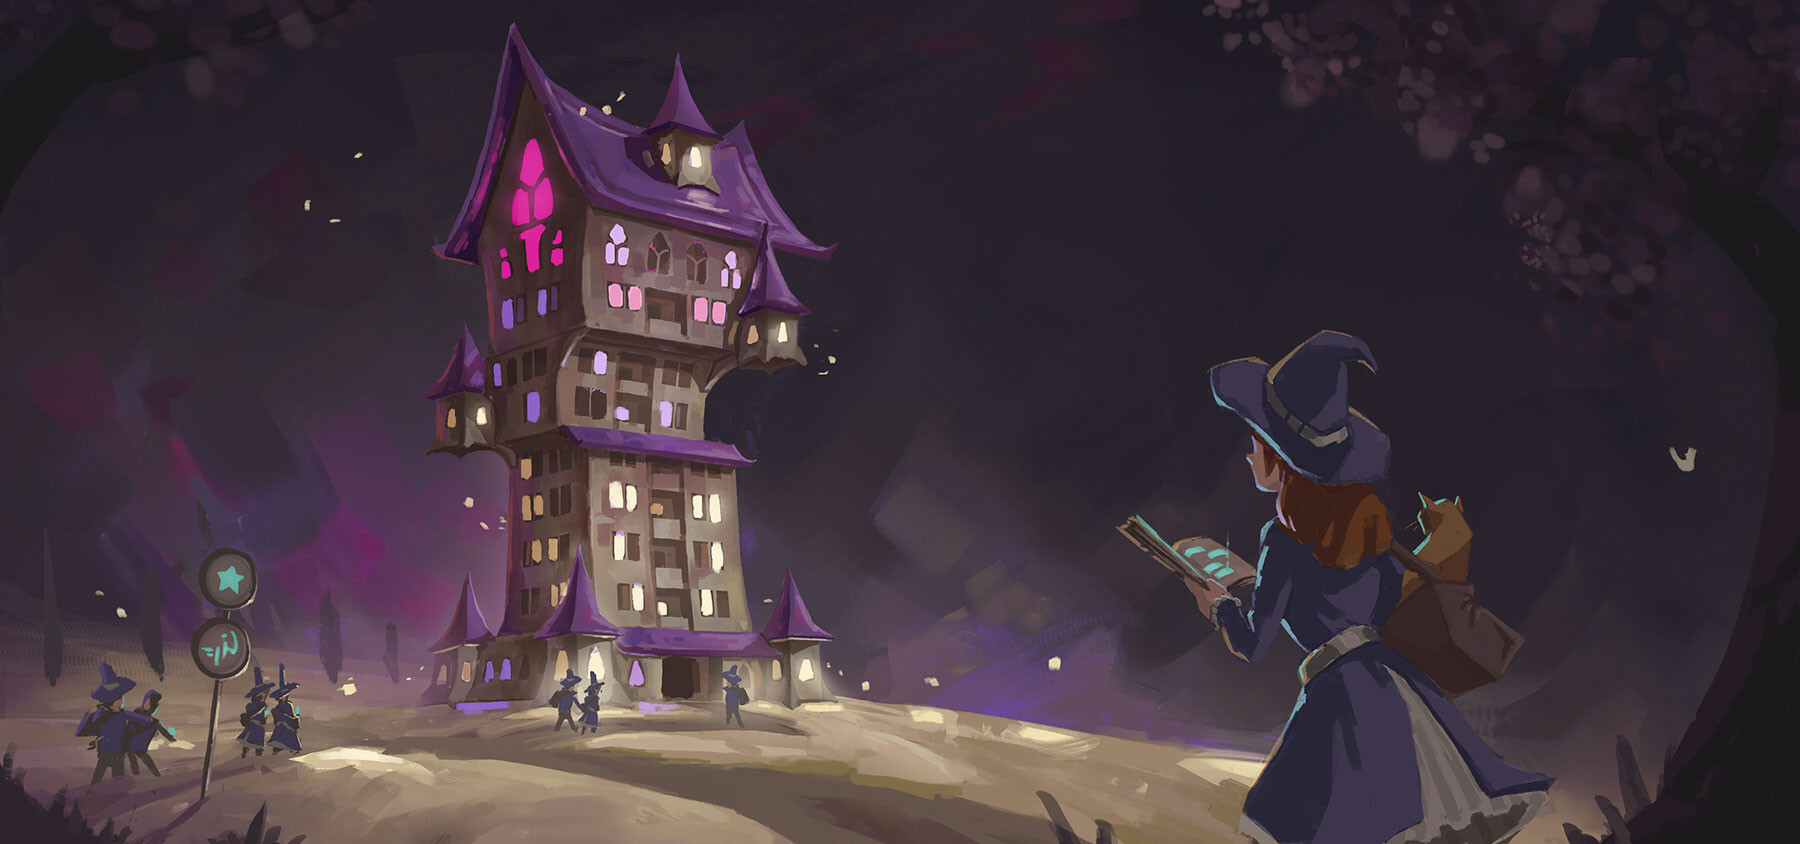
\includegraphics[width=0.6\linewidth]{images/setting-school.jpg}
    \caption{University of Wizardry and Applied Magics by Vadym Stovbunskyi.\nocite{stovbunskyi_university_2019}}
\end{figure}

\begin{figure}[h!]
    \centering
    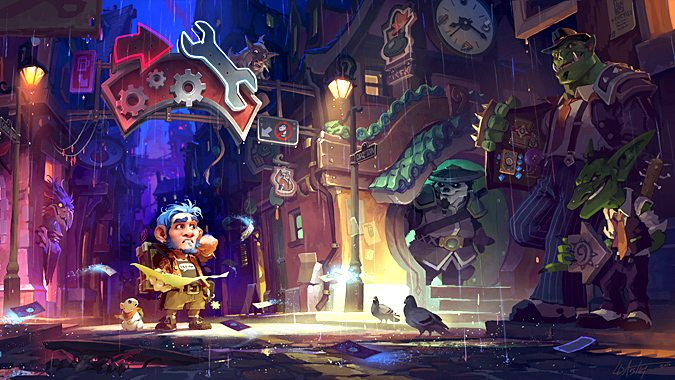
\includegraphics[width=0.6\linewidth]{images/setting-populated.jpg}
    \caption{Mean Streets Key Art by Blizzard Entertainment, Inc.\nocite{blizzard_entertainment_inc_mean_2016}}
\end{figure}